\chapter{Calcul littéral et équations}\label{ch:g8:equations}

L'année 7 a introduit les lettres et réduit des expressions simples
(\cref{ch:g7:literal}). Ce chapitre ajoute les deux compétences qui
rendent l'algèbre puissante~: \emph{développer} des \omterm{def:g2:mult:def}{produits} de
parenthèses, et \emph{résoudre des \omterm{def:g8:equations:def}{équations}} --- trouver le nombre
caché derrière la lettre.

\section{Développer}

\begin{theorem}[Distributivité simple et double]\label{thm:g8:equations:expand}
Pour tous nombres~:
\[
k(a + b) = ka + kb,
\qquad
(a + b)(c + d) = ac + ad + bc + bd .
\]
\end{theorem}

\begin{proof}
La première règle est \cref{thm:g7:priorities:distributivity} (signes
inclus~: $k$ et les termes peuvent être négatifs,
\cref{ch:g8:negprod}). Pour la seconde, appliquer la première règle
deux fois, en traitant $(c + d)$ comme un seul nombre~:
\[
(a + b)(c + d) = a(c + d) + b(c + d) = ac + ad + bc + bd .
\qedhere
\]
\end{proof}

\begin{example}\label{ex:g8:equations:expand}
Attention aux signes à chaque terme~:
\begin{align*}
3(2x - 5) &= 6x - 15, \\
-2(4x - 7) &= -8x + 14
&& \text{(un moins devant inverse les deux signes)}, \\
(x + 3)(x + 5) &= x^2 + 5x + 3x + 15 = x^2 + 8x + 15, \\
(2x - 1)(x - 4) &= 2x^2 - 8x - x + 4 = 2x^2 - 9x + 4 .
\end{align*}
\end{example}

\begin{omfigure}
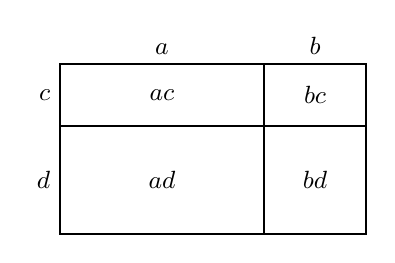
\begin{tikzpicture}[scale=0.72]
  \draw[thick] (0,0) rectangle (5.4,3.0);
  \draw[thick] (3.6,0) -- (3.6,3.0);
  \draw[thick] (0,1.9) -- (5.4,1.9);
  \node[font=\small] at (1.8,2.45) {$ac$};
  \node[font=\small] at (4.5,2.45) {$bc$};
  \node[font=\small] at (1.8,0.95) {$ad$};
  \node[font=\small] at (4.5,0.95) {$bd$};
  \node[above, font=\small] at (1.8,3.0) {$a$};
  \node[above, font=\small] at (4.5,3.0) {$b$};
  \node[left, font=\small] at (0,2.45) {$c$};
  \node[left, font=\small] at (0,0.95) {$d$};
\end{tikzpicture}

{\small Double distributivité comme \omterm{def:g6:measure:area}{aires}~: le rectangle
$(a+b) \times (c+d)$ se découpe en quatre rectangles plus petits ---
un par terme du développement.}
\end{omfigure}

\begin{method}[Développer et réduire]\label{met:g8:equations:reduce}
\begin{enumerate}
  \item Développer chaque \omterm{def:g2:mult:def}{produit}, en écrivant chaque terme avec son
        signe~;
  \item regrouper les termes semblables ($x^2$ avec $x^2$, $x$ avec
        $x$, nombres avec nombres)~;
  \item vérifier avec une valeur~: substituer par ex.\ $x = 2$ dans
        l'original et dans le résultat --- des résultats égaux
        attrapent la plupart des erreurs.
\end{enumerate}
\end{method}

\section{Résoudre des équations}

\begin{definition}[Équation]\label{def:g8:equations:def}
Une \emph{équation}\index{équation} est une égalité avec un nombre
inconnu, noté $x$ (ou toute autre lettre). La \emph{résoudre}, c'est
trouver toutes les valeurs de $x$ rendant l'égalité vraie --- les
\emph{solutions}.
\end{definition}

\begin{theorem}[Règles de la balance]\label{thm:g8:equations:balance}
Une \omterm{def:g8:equations:def}{équation} conserve exactement les mêmes solutions lorsque~:
\begin{enumerate}
  \item le même nombre est ajouté à (ou soustrait de) les deux
        membres~;
  \item les deux membres sont multipliés (ou divisés) par le même
        nombre \emph{non nul}.
\end{enumerate}
\end{theorem}
\admitted

\begin{omfigure}
\begin{tikzpicture}[scale=0.9]
  \draw[thick] (0,0) -- (0,0.5);
  \draw[thick] (-2.6,0.5) -- (2.6,0.5);
  \draw[thick] (-0.5,0) -- (0.5,0);
  \draw[thick] (-2.2,0.5) -- (-2.2,0.75);
  \draw[thick] (2.2,0.5) -- (2.2,0.75);
  \draw[omDef, fill=omDef!15] (-2.8,0.75) rectangle (-1.6,1.45);
  \node[font=\small] at (-2.2,1.1) {$x{+}3$};
  \draw[omThm, fill=omThm!15] (1.75,0.75) rectangle (2.65,1.45);
  \node[font=\small] at (2.2,1.1) {$8$};
  \node[below, font=\small] at (0,-0.25)
    {ôter $3$ des deux plateaux~: $x = 5$};
\end{tikzpicture}

{\small Une \omterm{def:g8:equations:def}{équation} est une balance en équilibre~: tout ce qui est
fait à un plateau doit l'être à l'autre, et l'équilibre ---
l'égalité --- survit.}
\end{omfigure}

\begin{method}[Résoudre une équation du premier degré]\label{met:g8:equations:solve}
\begin{enumerate}
  \item Développer et réduire chaque membre si besoin~;
  \item ajouter ou soustraire des deux côtés pour rassembler les
        termes en $x$ d'un côté, les nombres purs de l'autre~;
  \item réduire, puis diviser les deux membres par le coefficient de
        $x$~;
  \item \emph{vérifier} en substituant la valeur trouvée dans
        l'\omterm{def:g8:equations:def}{équation} originale.
\end{enumerate}
\end{method}

\begin{example}\label{ex:g8:equations:solve}
Résoudre $7x - 5 = 4x + 16$~:
\begin{align*}
7x - 5 &= 4x + 16 \\
7x - 4x &= 16 + 5
&& \text{(ajouter $5$, soustraire $4x$, des deux côtés)} \\
3x &= 21 \\
x &= 7 && \text{(diviser les deux membres par 3).}
\end{align*}
Vérification~: membre de gauche $7 \times 7 - 5 = 44$~; membre de
droite $4 \times 7 + 16 = 44$. La solution est $7$.
\end{example}

\begin{example}[Avec parenthèses et négatifs]\label{ex:g8:equations:brackets}
Résoudre $3(x - 4) = 5 - 2(x + 1)$~:
\begin{align*}
3x - 12 &= 5 - 2x - 2 && \text{(développer les deux membres)} \\
3x - 12 &= 3 - 2x && \text{(réduire)} \\
5x &= 15 && \text{(ajouter $2x + 12$ des deux côtés)} \\
x &= 3 .
\end{align*}
Vérification~: $3(3 - 4) = -3$ et $5 - 2(3+1) = 5 - 8 = -3$. \quad
Solution~: $3$.
\end{example}

\begin{method}[Résoudre un problème par une équation]\label{met:g8:equations:problem}
\begin{enumerate}
  \item Choisir l'inconnue~: «~soit $x$ \dots~» (la quantité demandée,
        ou une quantité plus simple qui s'y rattache)~;
  \item traduire l'histoire en une \omterm{def:g8:equations:def}{équation}~;
  \item la résoudre~;
  \item interpréter~: répondre à la question d'origine en une phrase,
        avec les unités, et vérifier la réponse face à l'histoire.
\end{enumerate}
\end{method}

\begin{example}\label{ex:g8:equations:problem}
Lucas a $4$ ans de plus que sa sœur~; ensemble leurs âges somment à
$26$. Soit $x$ l'âge de la sœur~; alors Lucas a $x + 4$, et
\[
x + (x + 4) = 26
\ \Longrightarrow\
2x + 4 = 26
\ \Longrightarrow\
2x = 22
\ \Longrightarrow\
x = 11 .
\]
La sœur a $11$ ans, Lucas $15$. Vérification~: $11 + 15 = 26$ et
$15 - 11 = 4$.
\end{example}

\section{Ordre et inégalités}

\begin{proposition}[Opérations et ordre]\label{prop:g8:equations:order}
Ajouter le même nombre aux deux membres d'une inégalité la conserve~;
multiplier les deux membres par un nombre \emph{positif} la conserve~;
multiplier par un nombre \emph{négatif} la \emph{renverse}~:
\[
2 < 5 \ \text{ mais }\ (-1) \times 2 > (-1) \times 5 .
\]
\end{proposition}
\admitted

\begin{example}\label{ex:g8:equations:inequality}
Résoudre $5 - 2x \leq 11$~: soustraire $5$ des deux côtés,
$-2x \leq 6$~; diviser par $-2$ \emph{et renverser}~: $x \geq -3$.
Tous les nombres supérieurs ou égaux à $-3$ sont solutions --- une
\omterm{def:g8:equations:def}{équation} a d'ordinaire une solution, une inégalité en a toute une
demi-droite.
\end{example}

\section{Exercices}

\begin{exercise}[$\star$]\label{exo:g8:equations:1}
Développer et réduire~:
\[
5(2x + 3), \qquad
-3(4x - 1), \qquad
2(3x - 2) + 4(x + 5).
\]
\end{exercise}

\begin{exercise}[$\star$]\label{exo:g8:equations:2}
Développer et réduire~:
\[
(x + 2)(x + 7), \qquad
(3x + 1)(2x - 5), \qquad
(x - 4)(x - 6).
\]
\end{exercise}

\begin{exercise}[$\star$]\label{exo:g8:equations:3}
$x = 3$ est-il solution de $4x - 5 = 7$~? De $2x + 1 = x + 4$~? De
$x^2 = 6x - 9$~? (Substituer et comparer les deux membres.)
\end{exercise}

\begin{exercise}[$\star$]\label{exo:g8:equations:4}
Résoudre, avec une vérification~:
\[
x + 9 = 4, \qquad
5x = -35, \qquad
\frac{x}{3} = 8, \qquad
2x - 7 = 13 .
\]
\end{exercise}

\begin{exercise}[$\star$]\label{exo:g8:equations:5}
Résoudre~:
\[
6x + 5 = 2x + 25, \qquad
9 - 4x = x - 11, \qquad
3(x + 2) = 2x + 11 .
\]
\end{exercise}

\begin{exercise}[$\star$]\label{exo:g8:equations:6}
Résoudre $4(2x - 3) = 5(x + 6)$, en développant d'abord, et vérifier
la solution.
\end{exercise}

\begin{exercise}[$\star$]\label{exo:g8:equations:7}
Traduire et résoudre~: «~le triple d'un nombre, diminué de $8$, vaut
$19$~»~; «~le double d'un nombre augmenté de $5$ égale le nombre
augmenté de $12$~».
\end{exercise}

\begin{exercise}[$\star\star$]\label{exo:g8:equations:8}
La longueur d'un rectangle dépasse de $5$ cm sa largeur, et son
\omterm{def:g6:measure:perimeter}{périmètre} est $58$ cm. Soit $x$ la largeur~: écrire une \omterm{def:g8:equations:def}{équation}, la
résoudre et donner les deux dimensions.
\end{exercise}

\begin{exercise}[$\star\star$]\label{exo:g8:equations:9}
Trois nombres entiers consécutifs ont pour \omterm{def:g1:addition:def}{somme} $141$. Appeler le
milieu $n$ et trouver les trois.
\end{exercise}

\begin{exercise}[$\star\star$]\label{exo:g8:equations:10}
Résoudre les inégalités et décrire les solutions~:
\[
3x + 4 > 19, \qquad
7 - 2x \geq 1, \qquad
5(x - 1) < 2x + 7 .
\]
\end{exercise}

\begin{exercise}[$\star\star$]\label{exo:g8:equations:11}
Mia a $140$ euros d'économies et ajoute $15$ euros chaque mois~; Tom
a $200$ euros et ajoute $10$ euros chaque mois. Après combien de mois
Mia aura-t-elle strictement plus que Tom~? (Mettre en place une
inégalité.)
\end{exercise}

\begin{exercise}[$\star\star\star$]\label{exo:g8:equations:12}
Résoudre l'\omterm{def:g8:equations:def}{équation} $\dfrac{x + 3}{4} = \dfrac{2x - 1}{5}$.
(Multiplier les deux membres par $20$, le \omterm{def:g4:fractions:def}{dénominateur} commun, puis
procéder comme d'habitude~; vérifier la solution dans l'\omterm{def:g8:equations:def}{équation}
originale.)
\end{exercise}

\section{Problème~: les identités remarquables et l'escalier des
nombres impairs}

\begin{problem}[{Devoir maison --- $(a+b)^2$, $(a-b)^2$,
$(a+b)(a-b)$, et la somme $1 + 3 + 5 + \dots + (2n-1) = n^2$}]
\label{pb:g8:equations:1}
Trois développements reviennent si souvent que l'algèbre les connaît
par cœur~: on les appelle les \emph{identités remarquables}. Ce
problème les établit à partir de la double distributivité
(\cref{thm:g8:equations:expand}), en fait un pouvoir de calcul
mental, s'en sert pour démontrer un beau résultat sur les \omterm{def:g3:numbers:evenodd}{nombres
impairs}, et s'achève en résolvant des \omterm{def:g8:equations:def}{équations} d'un genre tout
nouveau~: des \omterm{def:g8:equations:def}{équations} contenant un carré.

\medskip
\noindent\textbf{Partie I --- Les trois identités.}
\begin{enumerate}
  \item Développer $(a + b)^2 = (a + b)(a + b)$ et réduire, pour
        démontrer que
        \[
        (a + b)^2 = a^2 + 2ab + b^2 .
        \]
  \item Démontrer de même les deux compagnes~:
        \[
        (a - b)^2 = a^2 - 2ab + b^2,
        \qquad
        (a + b)(a - b) = a^2 - b^2 .
        \]
  \item Dessiner un carré de côté $a + b$, partager chaque côté en
        $a$ et $b$, et découper le carré en quatre morceaux. Quel
        terme de la première identité chaque partie du dessin
        représente-t-elle~?
  \item Calcul mental~: utiliser les identités pour calculer, sans
        poser aucune multiplication,
        \[
        101^2, \qquad 99^2, \qquad 49 \times 51 .
        \]
  \item Un piège classique~: Zoé écrit «~$(a + b)^2 = a^2 + b^2$~».
        Tester sa formule avec $a = 3$, $b = 4$, et expliquer sur le
        dessin de la question 3 quels morceaux exactement sa formule
        oublie.
\end{enumerate}

\medskip
\noindent\textbf{Partie II --- L'escalier des \omterm{def:g3:numbers:evenodd}{nombres impairs}.}
\begin{enumerate}[resume]
  \item Calculer $1$, puis $1 + 3$, puis $1 + 3 + 5$, puis
        $1 + 3 + 5 + 7$, puis $1 + 3 + 5 + 7 + 9$. Que remarque-t-on
        sur les résultats~?
  \item Expliquer pourquoi le $n$-ième \omterm{def:g3:numbers:evenodd}{nombre impair} vaut $2n - 1$
        (vérification~: $n = 1, 2, 3$ donnent $1, 3, 5$).
  \item Utiliser une identité de la partie I pour développer et
        réduire $(n + 1)^2 - n^2$. Quel rapport le résultat a-t-il
        avec la question 7~?
  \item La question 8 dit ceci~: pour passer d'un carré de côté $n$
        à un carré de côté $n + 1$, on ajoute exactement le \omterm{def:g3:numbers:evenodd}{nombre
        impair} suivant de cases unités --- une bordure en L le long
        de deux côtés, plus le coin. En partant de $1 = 1^2$ et en
        faisant grandir le carré couche par couche, expliquer
        pourquoi
        \[
        1 + 3 + 5 + \dots + (2n - 1) = n^2 :
        \]
        la \omterm{def:g1:addition:def}{somme} des $n$ premiers \omterm{def:g3:numbers:evenodd}{nombres impairs} est le $n$-ième
        carré.
  \item En déduire, sans les additionner un à un~: la valeur de
        $1 + 3 + 5 + \dots + 99$~; et combien de \omterm{def:g3:numbers:evenodd}{nombres impairs},
        à partir de $1$, totalisent exactement $400$.
\end{enumerate}

\medskip
\noindent\textbf{Partie III --- Des \omterm{def:g8:equations:def}{équations} avec un carré.}
\begin{enumerate}[resume]
  \item Reconnaître une identité remarquable dans $x^2 + 6x + 9$, et
        résoudre l'\omterm{def:g8:equations:def}{équation} $x^2 + 6x + 9 = 0$.
  \item Expliquer, à l'aide de la règle des signes et des distances
        du~\cref{thm:g8:negprod:rules}, pourquoi un \omterm{def:g2:mult:def}{produit} de deux
        nombres ne peut être nul \emph{que si} l'un des deux
        facteurs est nul. S'en servir pour résoudre
        $(x - 2)(x + 5) = 0$.
  \item Résoudre $x^2 = 49$ en ramenant tout d'un même côté et en
        factorisant $x^2 - 49$ à l'aide de la troisième identité.
        Combien de solutions cette \omterm{def:g8:equations:def}{équation} a-t-elle --- et en quoi
        cela diffère-t-il de toutes les \omterm{def:g8:equations:def}{équations} résolues jusqu'ici
        dans ce chapitre~?
  \item Dans \cref{exo:g8:equations:3}, on a vérifié que $x = 3$ est
        solution de $x^2 = 6x - 9$. Montrer que c'est la
        \emph{seule}~: ramener tout d'un même côté, reconnaître une
        identité, et conclure.
  \item Bouquet final~: calculer $2026^2 - 2025^2$ de tête, et
        expliquer à l'aide d'une identité pourquoi la \omterm{ex:g1:subtraction:difference}{différence} de
        deux carrés consécutifs est toujours la \omterm{def:g1:addition:def}{somme} des deux
        nombres --- c'est la question 8 à nouveau.
\end{enumerate}
\end{problem}
